\chapter{Analysis techniques}

\section{General strategy for searching for four top quarks}

The LHC has been said to be a ``top factory'' due to the large cross sections for \ttbar production at 8 TeV and 13 TeV, 253~pb and 831~pb respectively. Hence most analyses within the CMS collaboration which work on top quark physics study \ttbar production. Each of the top quarks will decay to a W boson and a b quark and the final state of the process in the detector is defined by whether the W boson decays leptonically into a lepton and neutrino or hadronically into two quark jets. The standard strategy is to require two b-jets to be present in the event and 0, 1, 2 leptons depending on the final state defined as \emph{all-hadronic}, \emph{semi-leptonic} and emph{dileptonic} respectively where 6, 4 or 2 jets are required. 

\begin{figure}[ht!]
\centering
    \includegraphics[width=0.5\textwidth]{images/Analysis/Ttbar_decay_channels.png}
    \caption{The possible decay channels for \ttbar production}
    \label{fig:ttbarDecay}
\end{figure}
%picture from wiki By Nazar Bartosik - http://bartosik.pp.ua/hep_sketches/tt_decay_channels, CC BY 4.0, https://commons.wikimedia.org/w/index.php?curid=49739344

Each selection of b-jets, leptons and total number of jets in the event will not be $100\%$ efficient which means not all \ttbar events will be captured within the selection. As the rate of \ttbar production is so high at the LHC, this is satisfactory as the total number of events is still high enough to have statistically relevant studies.\\

The strategy for selecting \tttt events while suppressing the selection of background processes is similar to the \ttbar selection but with the selection of additional two jets. The small cross section for \tttt production, 1.3~fb at 8~TeV and $\approx$9~fb at 13~TeV dictates the selection. It would be preferential to require 4 b-jets in the selection to obtain the highest signal to background ratio, however as b-tagging is $\approx70\%$ efficient, this would have a detrimental effect on the overall amount of \tttt found in the selection due to some b-jets not being identified correctly or being within the acceptance of the detector. Similarly, it is not possible to require the total number of jets in a \tttt final state as some of the jets may not be within the acceptance of the detector. However, it will be discussed in section~\ref{sec:Categorisation} how a looser selection can be used to an advance to constrain the main background process.

This thesis will mainly focus on the single lepton channel where only single muon and single electron final states are considered. As can be seen from~\ref{fig:ttttDecay}, the single lepton channel represents the largest branching ratio or four top quark decay channel. The dilepton channel, which has the second largest branching ratio will also briefly be discussed in chapter~\ref{c:Run2} as it was combined with the single lepton channel to achieve an increased sensitivity on the analysis. In the dilepton channel only final states with muons and electrons were considered.

\begin{figure}[ht!]
\centering
    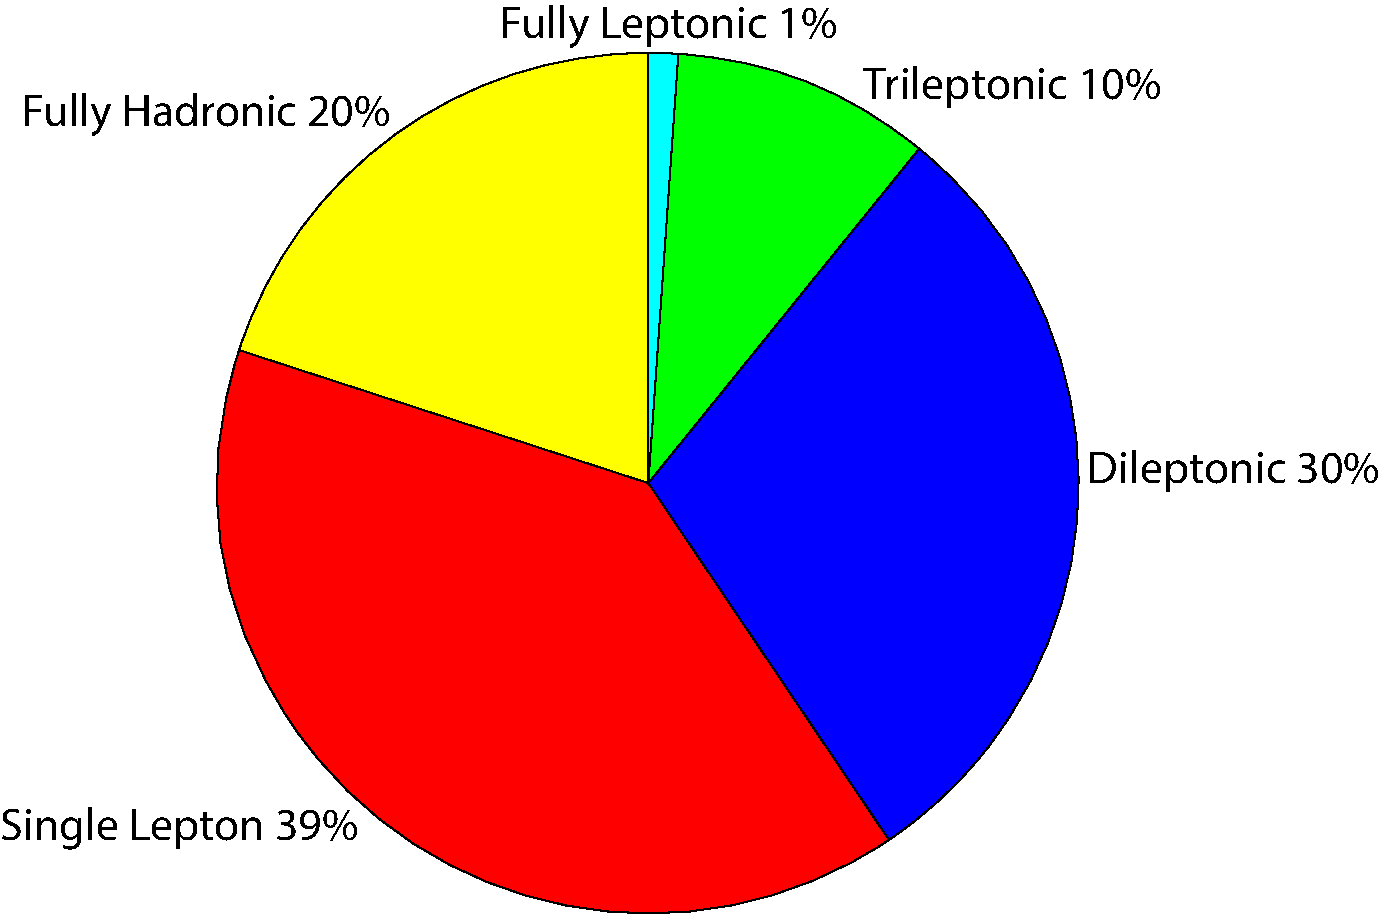
\includegraphics[width=0.5\textwidth]{images/Analysis/FourTopBR.pdf}
    \caption{The possible decay channels for \tttt production}
    \label{fig:ttttDecay}
\end{figure}




\section{Calibrations of the simulation}
\label{sec:Calibrations}
Many of the parameters which go into making simulation for each particle physics process are not precisely known therefore they are tuned to produce the simulation which best matches the data observed. This simulation will still have discrepancies from data which can be measured and accounted for by producing \emph{scale factors} which adjust the weight of each event in the simulation such that the overall distributions more closely match data. 


\subsection{Pileup reweighting}
\label{sec:pile-up}
The distribution of the number of primary vertices varies between data and simulation. This can be taken into account by looking at the number of events for each number of primary vertices in data and simulation and applying the scale factor, $SF_{PU}\left( i \right)$ to simulation, where \emph{i} is the number of vertices.

\begin{equation}
SF_{PU}\left( i \right) = \frac{N_{events}^{Data}}{  N_{events}^{simu}} 
\label{eqn:PUSF}
\end{equation}

\subsection{b tag modelling}

There are significant differences between b tag efficiencies measured by CMS in data and the efficiencies as measured in simulation. To account for this, a weight must be applied to the selected MC events in order to predict the correct event yield in data. The full method can be found in this reference~\cite{CMS-PAS-BTV-13-001}.

\subsection{Heavy flavour jet modelling}

There is a discrepancy between data and simulation in the tails of the \fxnote*{show unweighted}{distribution} of the number of b-tagged jets (\nbtags) which suggests that the amount of heavy flavour jets in \ttbar events is incorrectly simulated. The ratio of \heavyflavour was measured by CMS to be $2.2 \pm 0.3 \left( \textrm{stat.} \right) \pm 0.5 \left(\textrm{sys.} \right)\% $ ~\cite{CMS:2014yxa} at $\sqrt{s} =$ 8TeV. To incorporate this ratio into the analysis, the MC truth information of the \ttbar$+$jets MC sample is used to split the sample into \ttbb, \ttcc and \ttll, where l denotes light quarks and gluons (\cPqu, \cPqd, \cPqs, \cPg) . Weights are applied to each sub-sample to match the measured ratio whilst preserving the total number of \ttbar events. After this procedure is applied, the agreement between data and simulation in the \nbtags distribution is improved as can be seen in Fig~\ref{fig:datasimnbtags}.

\subsection{Lepton modelling}
Due to a difference between data and simulation in the efficiency of lepton identification and isolation, a weight is applied to events which is dependent on the selected leptons $\eta$, $\pt$ and lepton flavour.

\section{Multi-jet background estimation}
\label{sec:QCDbackground}
The presence of multi-jet events within the signal region defined by the baseline selection is investigated in this section. It is rare for multi-jet events to have a highly energetic undetectable particle. Therefore, the $\MET$ distributions for multi-jet events typically peak at \fxnote*{more specific?}{low values}. It can be seen from the MET distributions in Fig.~\ref{fig:datasimMET} that the data agrees well with the simulation at low values which suggests there are very few multi-jet events which pass the tight requirements in the baseline selection. Due to this small number of events, it is not possible to use multi-jet MC to estimate this background. In this case, a data-driven method known as the \fxnote*{ref?}{ABCD method} may be used. This method proceeds by selecting two uncorrelated variables from the object or baseline selection and defining three control regions (A,B,C) and one signal region (D) in the 2-dimensional phase space of these variables. The event variable \MET and the lepton variable RelIso were selected as they are \fxnote*{uncorrelated proof??}{uncorrelated} and the defined regions are shown below. Trigger requirements place an upper bound on the RelIso which restricts the region choice.\\











\section{Multi-variate analysis techniques}
\subsection{Boosted Decision Trees}
\label{sec:BDT}


\subsection{Reconstruction of hadronic top quarks}

\subsection{Event-level BDT}

\section{Limit setting}

\subsection{Categorisation}
\label{sec:Categorisation}




